\documentclass[11pt, a4paper]{article}
\usepackage[utf8]{inputenc}
\usepackage{a4wide}
\usepackage{anysize}
\usepackage[centertags]{amsmath}
\usepackage{amsfonts,amssymb,amsthm}
\usepackage{tikz}
\usetikzlibrary{positioning}
\usetikzlibrary{shapes}
\usepackage{graphicx}
\usepackage{placeins}   % to stop floats from floating
\usepackage[numbers]{natbib}    % so that natbib does not need author-year only numbers
\usepackage{wrapfig}
\usepackage{color}
\setcitestyle{square}
\renewcommand{\baselinestretch}{1.2} %line spacing
\marginsize{1.2in}{1.2in}{1in}{1in}  %left right top bottom
\title{Human Fall Detection Using Inertial Sensors}
\author{Simranjeet Singh (183076005), Sonali Shukla (184070014) \& Niraj N Sharma (184077001)}
\begin{document}
\pagenumbering{arabic}
\maketitle
\section*{Abstract}
In this project we developed a wearable human fall-detection system
intended for the elderly. On detecting a fall, the system sends an
emergency SMS using the wearer's bluetooth enabled smartphone to a
caregiver. The system uses a GY-87 inertial sensor integrated with an
Arduino Nano micro-controller.

\section{Problem Statement}
Falls are a significant source of injury for the elderly. This wearable
device aims to detect a fall by detecting the change in accelerometer
output, before during and immediately after a fall. It also detects the
direction of the fall by combining readings from the accelerometer with
gyroscope output. The combination of readings from the two sensors using a
complementary filter results in more usable readings compared to
just the use of the accelerometer. The HC05 bluetooth module pairs the
wearable with the user's bluetooth enabled smartphone. In the event of a
fall the devices sends a message to the the smartphone which is loaded
with an application to convert the message into a SMS to a designated
caregiver.

\section{Literature Review}
\cite{Mubashir2013} is a comprehensive survey of recent fall detection
techniques which includes wearable based detection as well as detection
using ambient and vision sensors. Wearable based detection increasingly
gravitate towards accelerometer based techniques due to lower costs and
power efficiency of mems-based accelerometers. Accelerometer-based techniques usually consist of detecting a sudden change in the
acclerator output due to the fall-event.

\cite{Bourke2011} discusses appropriate filtering techniques to estimate
the vertical acceleration vector from a tri-axial accelerometer. The
readings from a tri-axial accelerometer cannot be used directly as they
tend to be very noisy and are also combined with the acceleration due to
the earth's gravity.

{\color{red} PCP's student's mtech thesis} used a LPF to filter the
accelerometer readings with a cut-off frequency of {\color{red} Hz}.

\cite{Wu2015} uses a threshold based technique combining readings from
the accelerometer and gyroscope to detect the fall-event.

\section{Approach}
The idea is to use the I2C interface to interface a GY-87 sensor to the
Arduino Nano's micro-controller. The GY-87 provides separate readings for each
axes of the accelerator and gyroscope sensors. These six separate readings are
combined using a complementary filter. Our fall detection algorithm works on
the output of the complementary filter, by identifying a fall when the values
cross a certain preset threshold. We then experimented with various regular
movements like walking, running (slowly), climbing stairs, sitting and
sleeping to find an appropriate threshold value below which a fall should not
be detected. In addition to comparing the combined accelro-gyro output against
the threshold, we also use declare that a fall has been detected only when the
gyroscope indicates that the orientation of the device has changed by at least
60 degrees.

\section{Hardware Setup}
Our hardware setup consists of four major components:
\begin{description}
   \item [GY-87] The GY-87 also known as the MPU-60X0 integrates a
      tri-axial accelerometer and gyroscope with on-chip ADCs to deliver
      digital outputs via an I2C interface to an off-chip controller. To
      a controller this device acts as a slave on the I2C. GY-87 also
      features an auxiliary I2C bus which it masters to integrate
      discrete sensors like magnetometers.

   \item [Arduino Nano] The Arduino Nano is a board based on the
      ATmega328P microcontroller. The ATmega328 has 32 KB, (also with 2
      KB used for the bootloader). We have chosen the Nano due to its
      small form factor as the device is meant to be a wearable.

   \item [HC05] The HC05 is a bluetooth to serial port module which
      communicates via UART. The bluetooth module communicates fall
      information to a bluetooth enabled smartphone

   \item [Power Supply] A 9V battery is used as the power supply on the
      wearable.
\end{description}

\begin{figure}[htb]
    \centering
    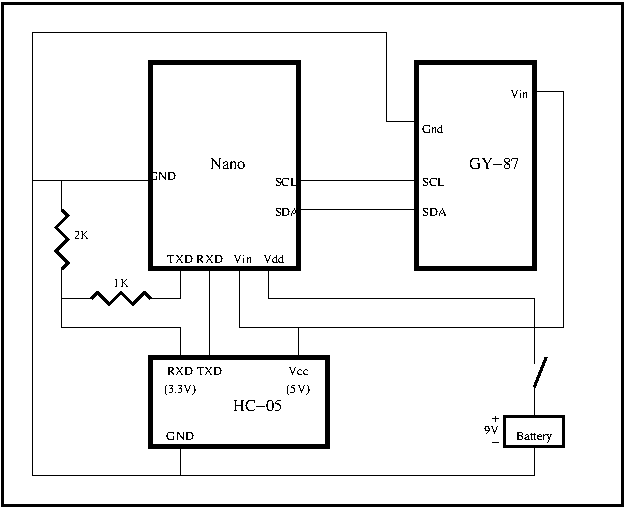
\includegraphics[width=\linewidth]{BD.pdf}
    \caption{Block Diagram}
    \label{fig:blk_diagram}
\end{figure}


\subsection{I2C and UART Integration}
The I2C is used to integrate the GY-87 with the ATmega328P. The GY-87 behaves
as a slave. 

\begin{figure}[htb]
    \centering
    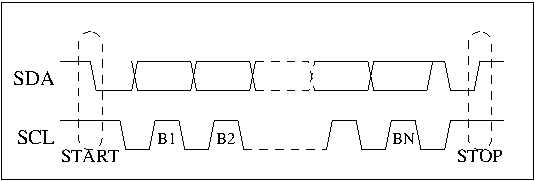
\includegraphics[width=\linewidth]{I2C_Timing.pdf}
    \caption{I2C Data Transfer}
    \label{fig:i2c_timing}
\end{figure}

\noindent The HC05 communicates with via a UART interface which is run at a
baud rate of 9600 baud.

\begin{figure}[htb]
    \centering
    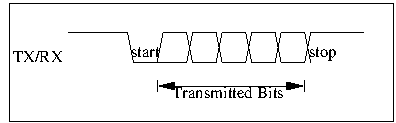
\includegraphics[width=\linewidth]{UART_Timing.pdf}
    \caption{UART Data Transfer}
    \label{fig:uart_timing}
\end{figure}

\subsection{GY87 Calibration and Integration}
Two experiments were conducted on the GY87 to calibrate it prior to
integration.

\subsubsection{Cube-mounted Measurements}
The GY-87 was mounted along the face of a thermocol cube. The cube itself was
placed on the surface of a flat table. The readings along the axis aligned to
the earth's gravitation field were verified to be as close to $\pm g$. This
experiment was repeated aligning each axis with g. The following readings were
recorded:

\begin{center}
   \begin{tabular}{llll}
      \hline
      Alignment Axis & A$_{x}$ & A$_{y}$ & A$_{z}$\\
      \hline
      X-Axis & $-9.8$ & $0.0$ & $0.0$ \\
      Y-Axis & $0.0$ & $-9.8$ & $0.0$ \\
      Z-Axis & $0.0$ & $0.0$ & $-9.8$ \\
      \hline
   \end{tabular}
\end{center}


\subsection{Power Supply}
During development the assembly was powered using the micro-usb connection to
the Arduino-Nano. Once we assembled the device as a wearable, we were using a
9V cell with a capacity of 400 mAH to power the device. The following table
lists the different devices and their peak current consumption:

\begin{center}
   \begin{tabular}{llll}
      \hline
      Device & Current Drawn (mA) \\
      \hline
      Arduino Nano & $2.4$ \\
      GY-87 Sensors & $3.9$ \\
      LEDs (4) & $16.0$ & \\
      HC-05 & $30.0$ \\
      \hline
      Total & $53.3$ \\
      \hline
   \end{tabular}
\end{center}

\noindent So, the device can draw a peak current of $53.3$ mA. At this
consumption, a 9V cell will last for about $7.50$ hours.

\section{Software}
Algorithm.
Flow diagram: sampling, lpf, hpf, complementary.

\section{Investigations}


\section{Test Procedure}
We tested the device both with normal movements, such as walking, sitting,
jumping and sleeping. The tests also included transitions between these
movements as the transition points were more interesting from our
application's point-of-view. The following are plots of {\color{red}
something, something and something-else} for each movement.

\noindent Wearer walked at a normal pace during this test. 
\begin{figure}
    \centering
    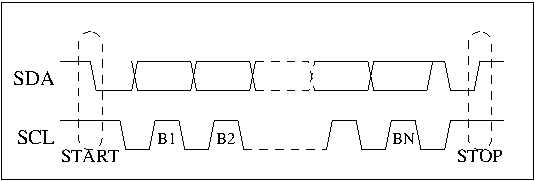
\includegraphics[width=\linewidth]{I2C_Timing.pdf}
    \caption{Plot: Walking}
    \label{fig:walking}
\end{figure}

\noindent This test was conducted when the wearer sat into a short chair from a
standing position and stood up again.
\begin{figure}
    \centering
    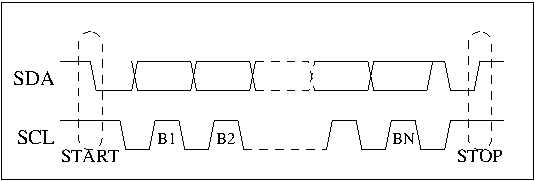
\includegraphics[width=\linewidth]{I2C_Timing.pdf}
    \caption{Plot: Sitting-Standing}
    \label{fig:sitting_standing}
\end{figure}

\noindent This test was conducted when the wearer was jumping in place. This
action most closely resembles a fall, and the test was conducted to ensure our
thresholding was correct.
\begin{figure}
    \centering
    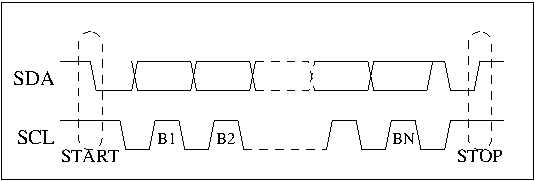
\includegraphics[width=\linewidth]{I2C_Timing.pdf}
    \caption{Plot: Jumping}
    \label{fig:jumping}
\end{figure}

\noindent This test was conducted when the wearer was lying down and suddenly
got up.
\begin{figure}
    \centering
    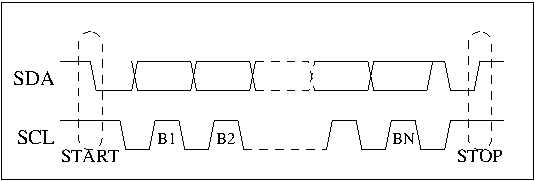
\includegraphics[width=\linewidth]{I2C_Timing.pdf}
    \caption{Plot: Sleeping-Waking}
    \label{fig:sleeping}
\end{figure}

\section{Test Results}
with plots and tables (appendices, if necessary).

\section{Conclusion}
suggestions for further improvement.


\bibliographystyle{ieeetr}
\bibliography{reference-papers}
\end{document}
